%%%%%%%%%%%%%%%%%%%%%%%%%%%%%%%%%%%%%%%%%%%%%%%%%%%%%%%%%%%%%%%%%%%%%
% LaTeX Template: Project Titlepage Modified (v 0.1) by rcx
%
% Original Source: http://www.howtotex.com
% Date: February 2014
% 
% This is a title page template which be used for articles & reports.
% 
% This is the modified version of the original Latex template from
% aforementioned website.
% 
%%%%%%%%%%%%%%%%%%%%%%%%%%%%%%%%%%%%%%%%%%%%%%%%%%%%%%%%%%%%%%%%%%%%%%

\documentclass[11pt]{report}
\usepackage[a4paper]{geometry}
\usepackage[myheadings]{fullpage}
\usepackage{fancyhdr}
\usepackage{lastpage}
\usepackage{graphicx, wrapfig, subcaption, setspace, booktabs}
\usepackage[T1]{fontenc}
\usepackage[font=small, labelfont=bf]{caption}
\usepackage{fourier}
\usepackage[protrusion=true, expansion=true]{microtype}
\usepackage[english]{babel}
\usepackage{sectsty}
\usepackage{url, lipsum}
\usepackage{amsmath}

\newcommand{\HRule}[1]{\rule{\linewidth}{#1}}
\onehalfspacing
\setcounter{tocdepth}{5}
\setcounter{secnumdepth}{5}

%-------------------------------------------------------------------------------
% HEADER & FOOTER
%-------------------------------------------------------------------------------
\pagestyle{fancy}
\fancyhf{}
\setlength\headheight{15pt}
\fancyhead[L]{Terrence Ho}
\fancyhead[R]{Experiment 4}
\fancyfoot[R]{Page \thepage\ of \pageref{LastPage}}
%-------------------------------------------------------------------------------
% TITLE PAGE
%-------------------------------------------------------------------------------

\begin{document}

\title{ \normalsize \textsc{Physics 4AL}
        \\ [2.0cm]
        \HRule{0.5pt} \\
        \LARGE \textbf{\uppercase{Experiment 4: Momentum and Impulse}}
        \HRule{2pt} \\ [0.5cm]
        \vspace*{2\baselineskip}}

\date{}

\author{
        Terrence Ho | ID: 804793446 \\ 
        Date of Lab: May 9th, 2017 \\
        Lab Section: Tuesday, 5 P.M.\\
        T.A.: David Bauer\\
        Lab Partners: Robathan Harries}

\maketitle
\tableofcontents
\newpage

%-------------------------------------------------------------------------------
% Section title formatting
\sectionfont{\scshape}
%-------------------------------------------------------------------------------

%-------------------------------------------------------------------------------
% BODY
%-------------------------------------------------------------------------------
\section*{Discussion}
\addcontentsline{toc}{section}{Discussion}

\subsection*{Measured Values}
\addcontentsline{toc}{subsection}{Measured Values}

The mass of the glider used in the experiment was 203 $\pm$ 0.5 g.  The length
of the flag 38 $\pm$ 0.5 mm.  

\begin{figure}[h!]
    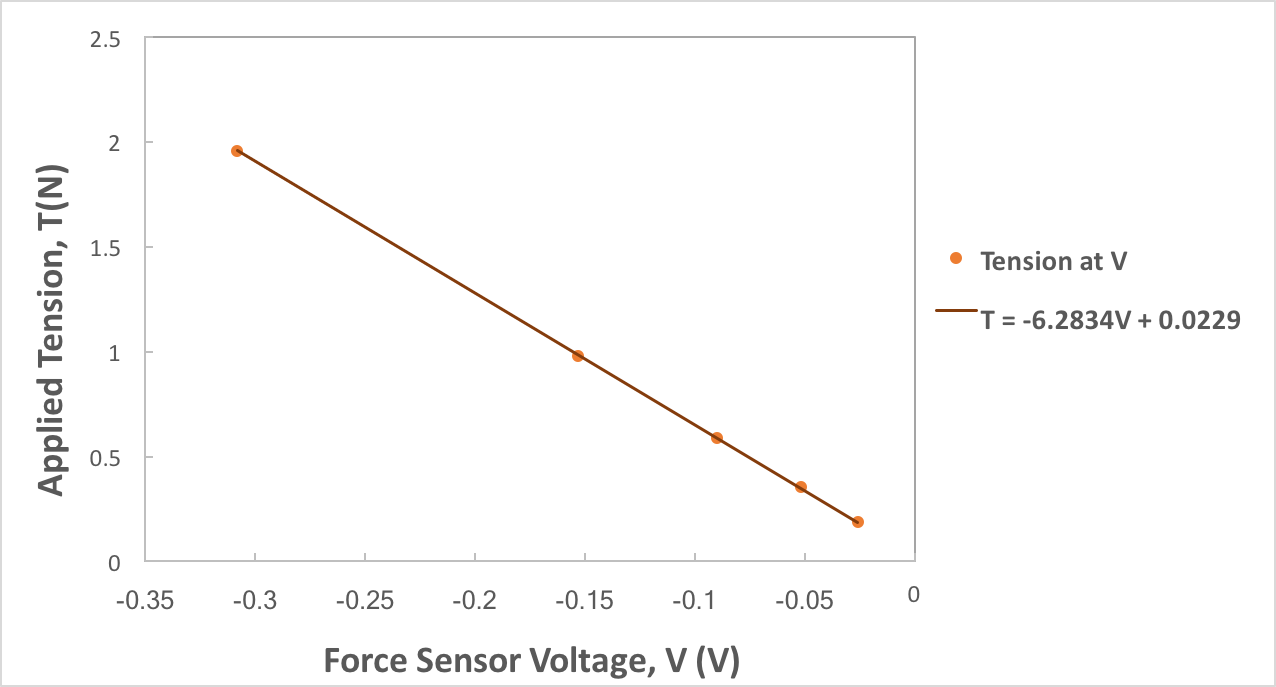
\includegraphics[width=\linewidth]{TensionVoltage.png}
    \captionsetup{labelformat=empty}
    \caption{\textbf{Figure 4.1  Voltage due to applied Tension.} The best fit
    line has the equation \(T = (-6.283 \pm 0.004)V + (0.023 \pm 0.002)\).  The
slope of the best fit line is the calibration constant: -6.283 $\pm$ 0.004 N/V.}
\addcontentsline{toc}{subsection}{Figure 4.1}
\end{figure}

\addcontentsline{toc}{subsection}{Table 4.1}
\begin{center}
    \begin{tabular}{| c | c | c |}
        \hline
        Trial & Initial Velocity (m/s) & Final Velocity (m/s) \\
        \hline
        1 & -0.1779 $\pm$ 0.0005 & 0.0821 $\pm$ 0.0005 \\
        \hline
        2 & -0.1415 $\pm$ 0.0005 & 0.0774 $\pm$ 0.0005 \\
        \hline
    \end{tabular}
\end{center}
\captionof*{table}{\textbf{Table 4.1} Initial and final velocities recorded by
the photogate for two trials.  Velocity heading towards the force sensor was
considered negative, and velocity directed away was positive.}

\subsection*{Impulse Calculation - Method 1}
\addcontentsline{toc}{subsection}{Impulse Calculation - Method 1}
Momentum, given by \(P\), is the product of mass \(m\) and velocity \(v\), or
\(P = mv\).  The change in momentum is known as impulse, or \(\Delta P = P_f -
P_i = m(v_f - v_i)\).  Using this formula, the velocities given in \textbf{Table
4.1}, and the mass of the glider, for Trial
one, the impulse $\Delta P_1$ = 0.0528 $\pm$ 0.0005 kg$\cdot$m/s.  For Trial
two, the impulse $\Delta P_2$ = 0.0408 $\pm$ 0.0005 kg$\cdot$m/s.

\begin{figure}[h!]
    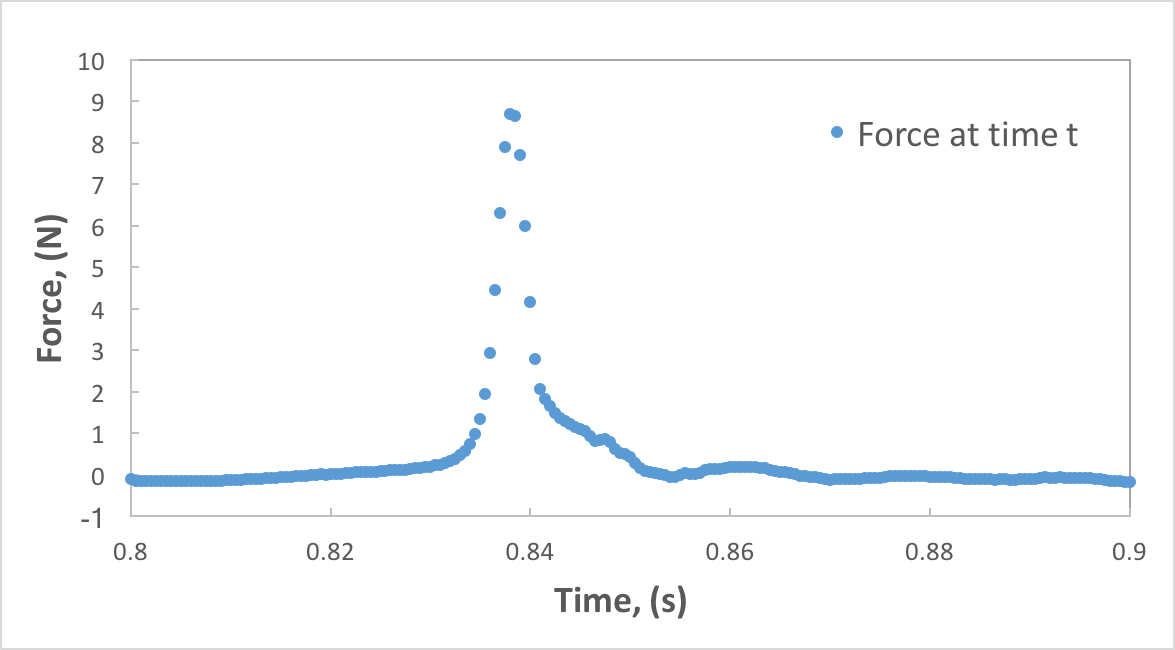
\includegraphics[width=\linewidth]{ForceTime1.png}
    \captionsetup{labelformat=empty}
    \caption{\textbf{Figure 4.2, Trial 1 of force of a moving glider against time.}
    This glider moved at a faster velocity than Trial 2.  The data points
represent the force sensor readings in Newtons at a specific time interval before and
after the collision.  The area under the curve of the peak represents the impulse of the collision.}
\addcontentsline{toc}{subsection}{Figure 4.2}
\end{figure}

\begin{figure}[h!]
    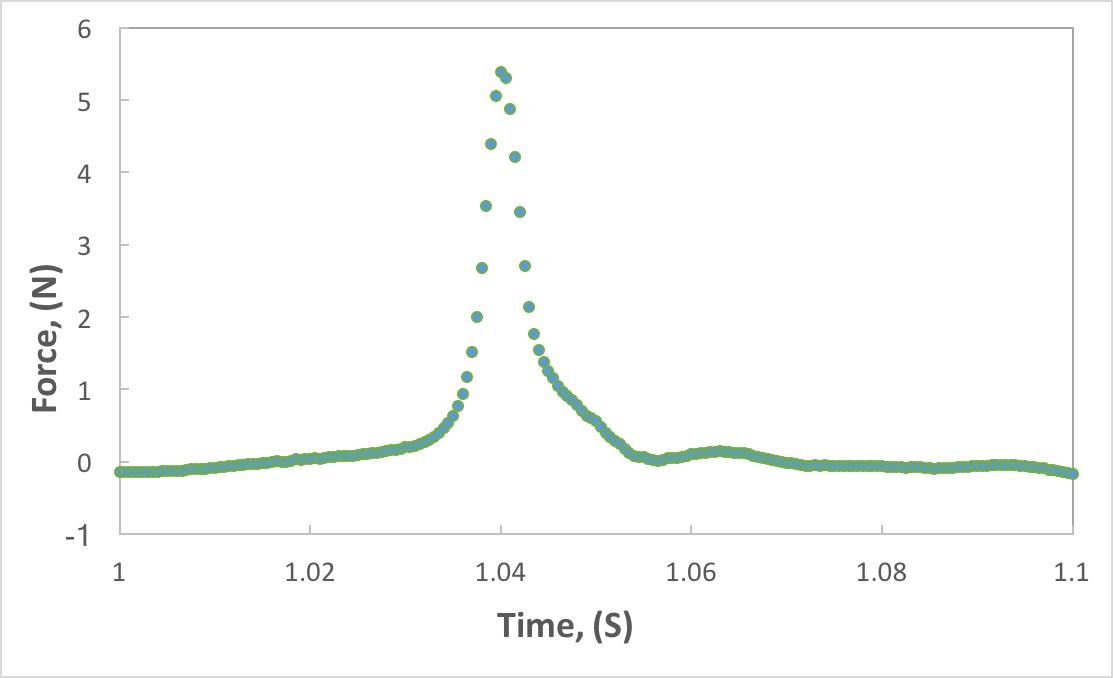
\includegraphics[width=\linewidth]{ForceTime2.png}
    \captionsetup{labelformat=empty}
    \caption{\textbf{Figure 4.3, Trial 2 of force of a moving glider against time.}
    This glider moved at a slower velocity compared to Trial 1. The data points
represent the force sensor readings in Newtons at a specific time interval before 
and after the collision.  The area under the curve of the peak represeents the impulse of the
collision.}
\addcontentsline{toc}{subsection}{Figure 4.3}
\end{figure}

\subsection*{Impulse Calculation - Method 2}
\addcontentsline{toc}{subsection}{Impulse Calculation - Method 2}
Impulse can also be known as the force \(F\) over time interval \(t\).  This can
be put into the form \(\Delta P = \int_{t_i}^{t_f} F(t)dt\).  We can approximate
this impulse using Riemann sums, or \(\Delta P \approx \Delta t
\sum_{i=1}^{n}\bar{F}(t_i)\), where $\Delta t$ is the time interval between each
data point, and \(\bar{F}(t_i)\) is the average force between $t_i$ and
$t_{i+1}$.  For our numerical integration $\Delta t$ was 0.0005 s, and \(\bar{F}(t_i) =
\frac{F(t_i) + F(t_{i+1})}{2}\).

\setlength{\parindent}{5ex}
To obtain our impulse calculations, we multipled the voltage read by the force
sensor by our calibration coefficient found previously in \textbf{Figure 4.1},
then subtracted the average background noise of the force sensor.  To calculate
our numerical integration, we needed to find the range where the force detected 
went above zero on both \textbf{Figures 4.2} and \textbf{4.3} (to signify the cart hitting the
force sensor). We the calculated the area under the curve with the formula involving
Riemann sums derived previously.  For Trial 1, \(\Delta P_1 = 0.04509 \pm
0.00003\) kg$\cdot$m/s, and for Trial 2, \(\Delta P_2 = 0.03701 \pm 0.00002\) kg$\cdot$m/s.  
The fractional uncertainty for the impulse is the same as the fractional 
uncertainty of the coefficient calibration.

\addcontentsline{toc}{subsection}{Table 4.2}
\begin{center}
    \begin{tabular}{| c | c | c |}
        \hline
        Trial & Impulse by Change in Momentum (kg$\cdot$m/s) & Impulse
        by Riemann Sums (kg$\cdot$m/s) \\
        \hline
        1 & 0.0528 $\pm$ 0.0005 & 0.04509 $\pm$ 0.00003 \\
        \hline
        2 & 0.0408 $\pm$ 0.0005 & 0.03701 $\pm$ 0.00002 \\
        \hline
    \end{tabular}
\end{center}
\captionof*{table}{\textbf{Table 4.2} Results for both trials and methods of
impulse calculation.}

We can see that calculating the impulse by Riemann Sums results in a lower
calculated impulse. We can attribute this error to the "ringing" of the force
sensor after it was struck by the cart, which would cause errors in the Reimann
sum calculation since impulse is still being exerted after it dipped back down
to zero in \textbf{Figures 4.2} and \textbf{4.3}.

\section*{Extra Credit}
\addcontentsline{toc}{section}{Extra Credit}
We tested two glider-to-glider collisions, one involving two bumpers and one
without bumpers at all.  For the bumper collision, the coefficient of
restitution was 0.3659, the initial energy was 0.0341 J, and the final energy
was 0.0046 J.  For the no-bumper collision, the COR was 0.5794, the initial
energy was 0.0584 J, and the final energy was 0.0198 J.  For the bumper
collision, the coefficient of restitution was lower, and the energy loss was
high, because only around 13\% of the energy remained after the collision.
Compared to the no bumper collision, which had 34\% of the initial energy,  
the energy loss was greater for the bumper collision.  Thus we can conclude with
a higher coefficient of restitution that the energy loss is less, because the
collision is closer to being an elastic collision.

\section*{Presentation}
\addcontentsline{toc}{section}{Presentation}

\subsection*{Introduction}
\addcontentsline{toc}{subsection}{Introduction}
Our experiment sought to prove that while energy is lost in inelastic collisions due to
friction, change in momentum, or impulse, is constant.  Impulse can be defined
in two different ways, by the amount of force acting over a certain time period,
or the change in momentum.
If both these ways of calculating impulse were equal, then we would have proved that impulse
is constant during a collision.  A glider with a flag on top was set up on an
air track with a force sensor at the end of a track and a photogate to track the
flag's movement.  The collision with the force sensor was monitored with the
photogate, and the velocities obtained by the photogate allowed us to calculate
impulse by change in momentum.  Force over time was measured with the force
sensor, and impulse was calculated by summing the force in the time interval of
the collision.  The two values obtained were compared to verify that the results
were close but outside the margin of error.

\subsection*{Methods}
\addcontentsline{toc}{subsection}{Methods}
\begin{figure}[h!]
    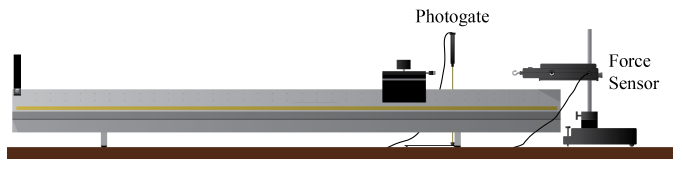
\includegraphics[width=\linewidth]{Figure44.png}
    \captionsetup{labelformat=empty}
    \caption{\textbf{Figure 4.4 Equipment for measuring the impulse of a glider
        colliding with force sensor.}
    The force sensor measures \(F(t)\) in volts, which allows you to gain an
independent measure of impulse by numerical integration.  The flag passes
through the photogate before and after the collision, which allows a different
way to measure initial and final momentum. Figure reproduced (with permission)
from Fig. 4.1 by Campbell, W. C. et al.$^1$}
\addcontentsline{toc}{subsection}{Figure 4.4}
\end{figure}

The first step of our experiment was to calibrate the force sensor.
We connected it to the PASCO machine and shifted the force sensor so that the
hook faced downwards, and hung masses of
various weights onto the hook to measure the voltage readings.  The masses we
used were 0.2 kg, 0.1 kg, 0.06 kg, 0.036 kg, and 0.019 kg. We graphed the
voltages measured and compared it to the force exerted by gravity on the masses,
to obtain the force sensor's calibration coefficient, which will be used to convert 
the voltages measured later to volts.

\setlength{\parindent}{5ex}
The mass of the glider with the flag was measured with a scale, and the length of the flag was
measured with a ruler.  The mass measurement will later be used to calculate
momentum of the glider.  Our equipment was set up in the same fashion as
\textbf{Figure 4.4}.  We connected the photogate and force sensor to the PASCO,
so the computer could record the velocity, time, and voltage of the force
sensor.  A preconfigured timer was chosen for the photogate, where speed was
chosen as the variable measured.  The length of the flag was typed in, so the
photogate knew how long the flag was and when to measure speed.  We kept the
same calibrations as before for the force sensor, but set the sample rate to
2kHz.  The measurements were measured in Continuous Mode on the PASCO machine.

We turned on the airtrack and slid the glider on the track twice towards
the force sensor.  When the glider passed through the photogate, the photogate
should record the speed of the glider twice, once before and after the glider
hits the force sensor.  The force sensor should be measuring voltage the whole
time during the trial, but should only see a spike in voltage when the glider
connects with the force sensor.  In the end, you should end up with three
columns of data, one for time, speed, and voltage.

We gave the glider less speed for the second trial compared
to the first trial.  Time of the trial, speed of the glider, and the voltage
were measured for each trial, and copied over to an Excel spreadsheet for
analysis.  

For uncertainty values of the experiment, we used $\pm$ 0.5 mm for the flag length and
$\pm$ 0.5 g for the mass of the glider, which are half the smallest precision of the
measurement devices.  We set the PASCO to measure voltage of the force sensor
within one digit of uncertainty (i.e. only the least significant digit measured
was flickering on the display).  The velocities measured had the same fractional
uncertainty as the calibration coefficient of the force sensor, which we can
find with regressional analysis on Excel.

To improve the accuracy of our experiment, we employed a few methods to
eliminate systematic errors.  The glider was put on an air track to reduce the
energy lost to friction.  The air track was set to be completely level, so that
the glider did not experience any acceleration due to gravity.  The average
background force detected by the force sensor was calculated and removed from
our final analysis, to avoid any systematic error by the force sensor.  
We also made sure to tare our force sensor before each trial, to ensure the 
background force remains as low as possible.  




\newpage
\section*{References}
\addcontentsline{toc}{section}{References}
\begin{enumerate}
    \item Campbell, W. C. et al. Physics 4AL: Mechanics Lab Manual (ver. April
        3, 2017). (Univ. California Los Angeles, Los Angeles, California).
\end{enumerate}
\end{document}



%-------------------------------------------------------------------------------
% REFERENCES
%-------------------------------------------------------------------------------
% \newpage
% \section*{References}
% \addcontentsline{toc}{section}{References}

% Anand, U., 2010. The Elusive Free Radicals, \textit{The Clinical Chemist,} [e-journal] Available at:<\url{http://www.clinchem.org/content/56/10/1649.full.pdf}> [Accessed 2 November 2013]
% \newline
% \newline

% Biology Forums, 2012. \textit{Normal glomerulus. Acute glomerulonephritis.} [online] Available at: <\url{http://biology-forums.com/index.php?action=gallery;sa=view;id=9284}> [Accessed 23 October 2013].
% \newline
% \newline

% Budisavljevic, M., Hodge, L., Barber, K., Fulmer, J., Durazo-Arvizu, R., Self, S., Kuhlmann, M., Raymond, J. and Greene, E., 2003. Oxidative stress in the pathogenesis of experimental mesangial proliferative glomerulonephritis, \textit{American Journal of Physiology - Renal Physiology,} 285(6), pp. 1138-1148.
% \newline
% \newline

% Chien, C., Lee, P., Chen, C., Ma, M., Lai, M. and Hsu, S., 2001. De Novo Demonstration and Co-localization of Free-Radical Production and Apoptosis Formation in Rat Kidney Subjected to Ischemia/Reperfusion, \textit{Journal of the American Society of Nephrology,} 12(5), pp. 973-982.
% \newline
% \newline

% Couser, W., 1993. Pathogenesis of glomerulonephritis, \textit{Kidney International Supplements,} 42, pp. 19-26.
% \newline
% \newline

% De Gasparo, M., 2002. Angiotensin II and nitric oxide interaction, \textit{Heart Failure Reviews,} [e-journal] Available at:<\url{http://www.ncbi.nlm.nih.gov/pubmed/12379820}> [Accessed 26 October 2013]
% \newline
% \newline

% Edinburgh Renal Education Pages, 2012. \textit{Glomerulonephritis} [online] Available at: <\url{http://www.edrep.org/pages/textbook/glomerulonephritis.php}> [Accessed 25 October 2013].
% \newline
% \newline

% Forbes, J., Coughlan, M. and Cooper, M., 2008. Oxidative Stress as a Major Culprit in Kidney Disease in Diabetes, \textit{Diabetes,} 57(6), pp. 1446-1454.
% \newline
% \newline

% Geeky Medics, 2010. \textit{Glomerulonephritis} [online] Available at: <\url{http://geekymedics.com/2010/10/27/glomerulonephritis/}> [Accessed 25 October 2013].
% \newline
% \newline

% Gryglewski, R., Palmer, R., Moncada, S., 1986. Superoxide anion is involved in the break­down of endothelium derived relaxing factor, \textit{Nature,} 320, pp. 454-456.
% \newline
% \newline

% Halliwell, B., 2001. Free Radicals and other reactive species in Disease, \textit{Encyclopedia of Life Sciences,} [e-journal] Available at:<\url{http://web.sls.hw.ac.uk/teaching/level4/bcm1_2/reading/oxidative_stress/files/Oxidative_stress.pdf}> [Accessed 19 October 2013]
% \newline
% \newline

% Huang, H., Patel, P. and Salahudeen, A., 2001. Lazaroid compounds prevent early but not late stages of oxidant-induced cell injury: potential explanation for the lack of efficacy of lazaroids in clinical trials, \textit{Pharmacological Research,} 41(1), pp. 55-61.
% \newline
% \newline

% Klinger, J., Abman, S. and Gladwin, M., 2013. Nitric Oxide Deficiency and Endothelial Dysfunction in Pulmonary Arterial Hypertension, \textit{American Journal of Respiratory and Critical Care Medicine,} 188(6), pp. 639-646.
% \newline
% \newline

% Lindemann, I., Boettcher, J., Oertel, K., Pasternack, R., Heine, A. and Klebe, G. 2012. Inhibitors of Transglutaminase 2: A therapeutic option in celiac disease, \textit{To be Published,} [e-journal + PDB structure] Available at:<\url{http://www.ebi.ac.uk/pdbe-srv/view/entry/3s3s/summary}> [Accessed 24 October 2013]
% \newline
% \newline

% Mayo Clinic, 2011. \textit{Glomerulonephritis} [online] Available at: <\url{http://www.mayoclinic.com/health/glomerulonephritis/DS00503/}> [Accessed 20 October 2013].
% \newline
% \newline

% McCord, J., Roy, R. and Schaffer, S., 1985. Free radicals and myocardial ischemia. The role of xanthine oxidase, \textit{Advances in myocardiology,} [e-journal] Available at:<\url{http://www.ncbi.nlm.nih.gov/pubmed/2982206}> [Accessed 24 October 2013]
% \newline
% \newline

% National Health Service, 2012. \textit{Causes of glomerulonephritis} [online] Available at: <\url{http://www.nhs.uk/Conditions/Glomerulonephritis/Pages/Causes.aspx}> [Accessed 20 October 2013].
% \newline
% \newline

% Niaudet, P., 2013. \textit{Overview of the pathogenesis and causes of glomerulonephritis in children.} [online] Available at: <\url{http://www.uptodate.com/contents/overview-of- \ the-pathogenesis-and-causes-of-glomerulonephritis-in-children}> [Accessed 21 October 2013].
% \newline
% \newline

% Ronco, P., 2013. \textit{Mechanisms of glomerular crescent formation.} [online] Available at: <\url{http://www.uptodate.com/contents/mechanisms-of-glomerular-crescent-formation}> [Accessed 21 October 2013].
% \newline
% \newline

% Rutchik, J., 2013. \textit{Toxic Neuropathy Clinical Presentation.} [online] Available at: <\url{http://emedicine.medscape.com/article/1175276-clinical#a0216}> [Accessed 26 October 2013].
% \newline
% \newline

% R\&D Systems, 2013. \textit{Technical Information. Ischemia/Reperfusion Injury.} [online] Available at: <\url{http://www.rndsystems.com/cb_detail_objectname_SP96_Ischemia.aspx}> [Accessed 28 October 2013].
% \newline
% \newline

% Salahudeen, A., 1999. Free Radicals in Kidney Disease and Transplantation, \textit{Saudi Journal of Kidney Diseases and Transplantation,} 10(2), pp. 137-143.
% \newline
% \newline

% Sarma, A., Mallick, A. and Ghosh, A., 2010. Free Radicals and Their Role in Different Clinical Conditions: An Overview, \textit{International Journal of Pharma Sciences and Research,} 1(3), pp. 182-192.
% \newline
% \newline

% Shah, S., Baliga, R., Rajapurkar, M. and Fonseca, V., 2007. Oxidants in Chronic Kidney Disease, \textit{Journal of the American Society of Nephrology,} 18(1), pp. 16-28.
% \newline
% \newline

% The University of Utah, Unknown. \textit{Glomerulonephritis} [online] Available at: <\url{http://library.med.utah.edu/WebPath/RENAHTML/RENALIDX.html#8}> [Accessed 25 October 2013].
% \newline
% \newline

% Wang, C. and Salahudeen, A., 1994. Cyclosporine nephrotoxicity: attenuation by an antioxidant -inhibitor of lipid peroxidation in-vitro and in-vivo, \textit{Transplantation,} 58, pp. 940-946.
% \newline
% \newline

% Wang, C. and Salahudeen, A., 1995. Lipid peroxidation accompanies cyclosporine nephrotoxicity: effects of vitamin E, \textit{Kidney International,} 47, pp. 927-934.
% \newline
% \newline

% Weiss, S., 1989. Tissue Destruction by Neutrophils, \textit{New England Journal of Medicine,} 320, pp. 365-376.
% \newline
% \newline



%-------------------------------------------------------------------------------
% SNIPPETS
%-------------------------------------------------------------------------------

%\begin{figure}[!ht]
%    \centering
%    \includegraphics[width=0.8\textwidth]{file_name}
%    \caption{}
%    \centering
%    \label{label:file_name}
%\end{figure}

%\begin{figure}[!ht]
%    \centering
%    \includegraphics[width=0.8\textwidth]{graph}
%    \caption{Blood pressure ranges and associated level of hypertension (American Heart Association, 2013).}
%    \centering
%    \label{label:graph}
%\end{figure}

%\begin{wrapfigure}{r}{0.30\textwidth}
%    \vspace{-40pt}
%    \begin{center}
%        \includegraphics[width=0.29\textwidth]{file_name}
%    \end{center}
%    \vspace{-20pt}
%    \caption{}
%    \label{label:file_name}
%\end{wrapfigure}

%\begin{wrapfigure}{r}{0.45\textwidth}
%    \begin{center}
%        \includegraphics[width=0.29\textwidth]{manometer}
%    \end{center}
%    \caption{Aneroid sphygmomanometer with stethoscope (Medicalexpo, 2012).}
%    \label{label:manometer}
%\end{wrapfigure}

%\begin{table}[!ht]\footnotesize
%    \centering
%    \begin{tabular}{cccccc}
%    \toprule
%    \multicolumn{2}{c} {Pearson's correlation test} & \multicolumn{4}{c} {Independent t-test} \\
%    \midrule    
%    \multicolumn{2}{c} {Gender} & \multicolumn{2}{c} {Activity level} & \multicolumn{2}{c} {Gender} \\
%    \midrule
%    Males & Females & 1st level & 6th level & Males & Females \\
%    \midrule
%    \multicolumn{2}{c} {BMI vs. SP} & \multicolumn{2}{c} {Systolic pressure} & \multicolumn{2}{c} {Systolic Pressure} \\
%    \multicolumn{2}{c} {BMI vs. DP} & \multicolumn{2}{c} {Diastolic pressure} & \multicolumn{2}{c} {Diastolic pressure} \\
%    \multicolumn{2}{c} {BMI vs. MAP} & \multicolumn{2}{c} {MAP} & \multicolumn{2}{c} {MAP} \\
%    \multicolumn{2}{c} {W:H ratio vs. SP} & \multicolumn{2}{c} {BMI} & \multicolumn{2}{c} {BMI} \\
%    \multicolumn{2}{c} {W:H ratio vs. DP} & \multicolumn{2}{c} {W:H ratio} & \multicolumn{2}{c} {W:H ratio} \\
%    \multicolumn{2}{c} {W:H ratio vs. MAP} & \multicolumn{2}{c} {\% Body fat} & \multicolumn{2}{c} {\% Body fat} \\
%    \multicolumn{2}{c} {} & \multicolumn{2}{c} {Height} & \multicolumn{2}{c} {Height} \\
%    \multicolumn{2}{c} {} & \multicolumn{2}{c} {Weight} & \multicolumn{2}{c} {Weight} \\
%    \multicolumn{2}{c} {} & \multicolumn{2}{c} {Heart rate} & \multicolumn{2}{c} {Heart rate} \\
%    \bottomrule
%    \end{tabular}
%    \caption{Parameters that were analysed and related statistical test performed for current study. BMI - body mass index; SP - systolic pressure; DP - diastolic pressure; MAP - mean arterial pressure; W:H ratio - waist to hip ratio.}
%    \label{label:tests}
%\end{table}
